

\PEEL{Les modèles intégrés sont sensibles aux choix éthiques des modélisateur.ices, ce qui a des conséquences importantes sur leur rôle dans la société.}{Taux d'actualisation, inégalités}{La prise en compte des inégalités (spatiales, sociales, temporelles) est un facteur majeur du niveau de dommage; la manière de les prendre en compte résulte de choix éthiques.}{On doit donc avoir un regard critique sur ces différents choix. }




\chapter*{Introduction}
\newrefsegment

\PEEL{Exposez l'idée principale ou l'argument que vous souhaitez développer dans cette partie.}{Fournissez des preuves, des données ou des citations qui soutiennent votre point.}{Expliquez en quoi les preuves que vous avez fournies sont pertinentes et comment elles appuient votre point.}{Faites le lien avec le sujet principal ou avec la section suivante de votre mémoire.}


%% Amorce

% réduction de l'incertitude => elle est désagréable donc on cherche toujours à la minimiser; 
% representer le monde le plus précisement possible => fantasme et ambition des sciences => La carte et le navigateur \cite{edenhofer_mapmakers_2014}. 



% Comment prendre les bonnes décisions face au changement climatique ? 



Longtemps, l'emphase a été mise sur la production de connaissance scientifique, pour s'assurer de l'existence de celui-ci, puis pour en mesurer avec toujours plus de précision l'ampleur et la vitesse. Cet effort de connaissance s'est aussi déployé par des tentatives de vulgarisation et de sensibilisation aux questions climatiques. Si ces efforts ont permis d'établir de manière presque consensuelle qu'il y avait un grave danger et une nécessité d'action face aux changements climatique, les mesures à prendre sont beaucoup moins claires. Deux exemples en témoignent assez bien. D'abord, la difficulté qu'ont les différentes nations à s'accorder sur une conduite commune, et ce, malgré l'ampleur de la crise et des moyens déployés (COPs, diplomatie climatique, etc.). Ensuite, la part qu'ont pris les sujets climatiques dans les positionnements politiques, comme nouveau marqueur : il faudrait plus de \textit{"justice sociale"}, ou encore lutter contre une \textit{"écologie punitive"}. \\

Une des difficultés réside dans l'incertitude qui entoure le changement climatique : d'abord, historiquement, autour de son existence; puis autour de son ampleur; aujourd'hui, autour des canaux par lesquels ces impacts vont se réaliser et leurs interactions avec des structures sociales par essence très complexes. 

\begin{figure}[h]
    \centering
    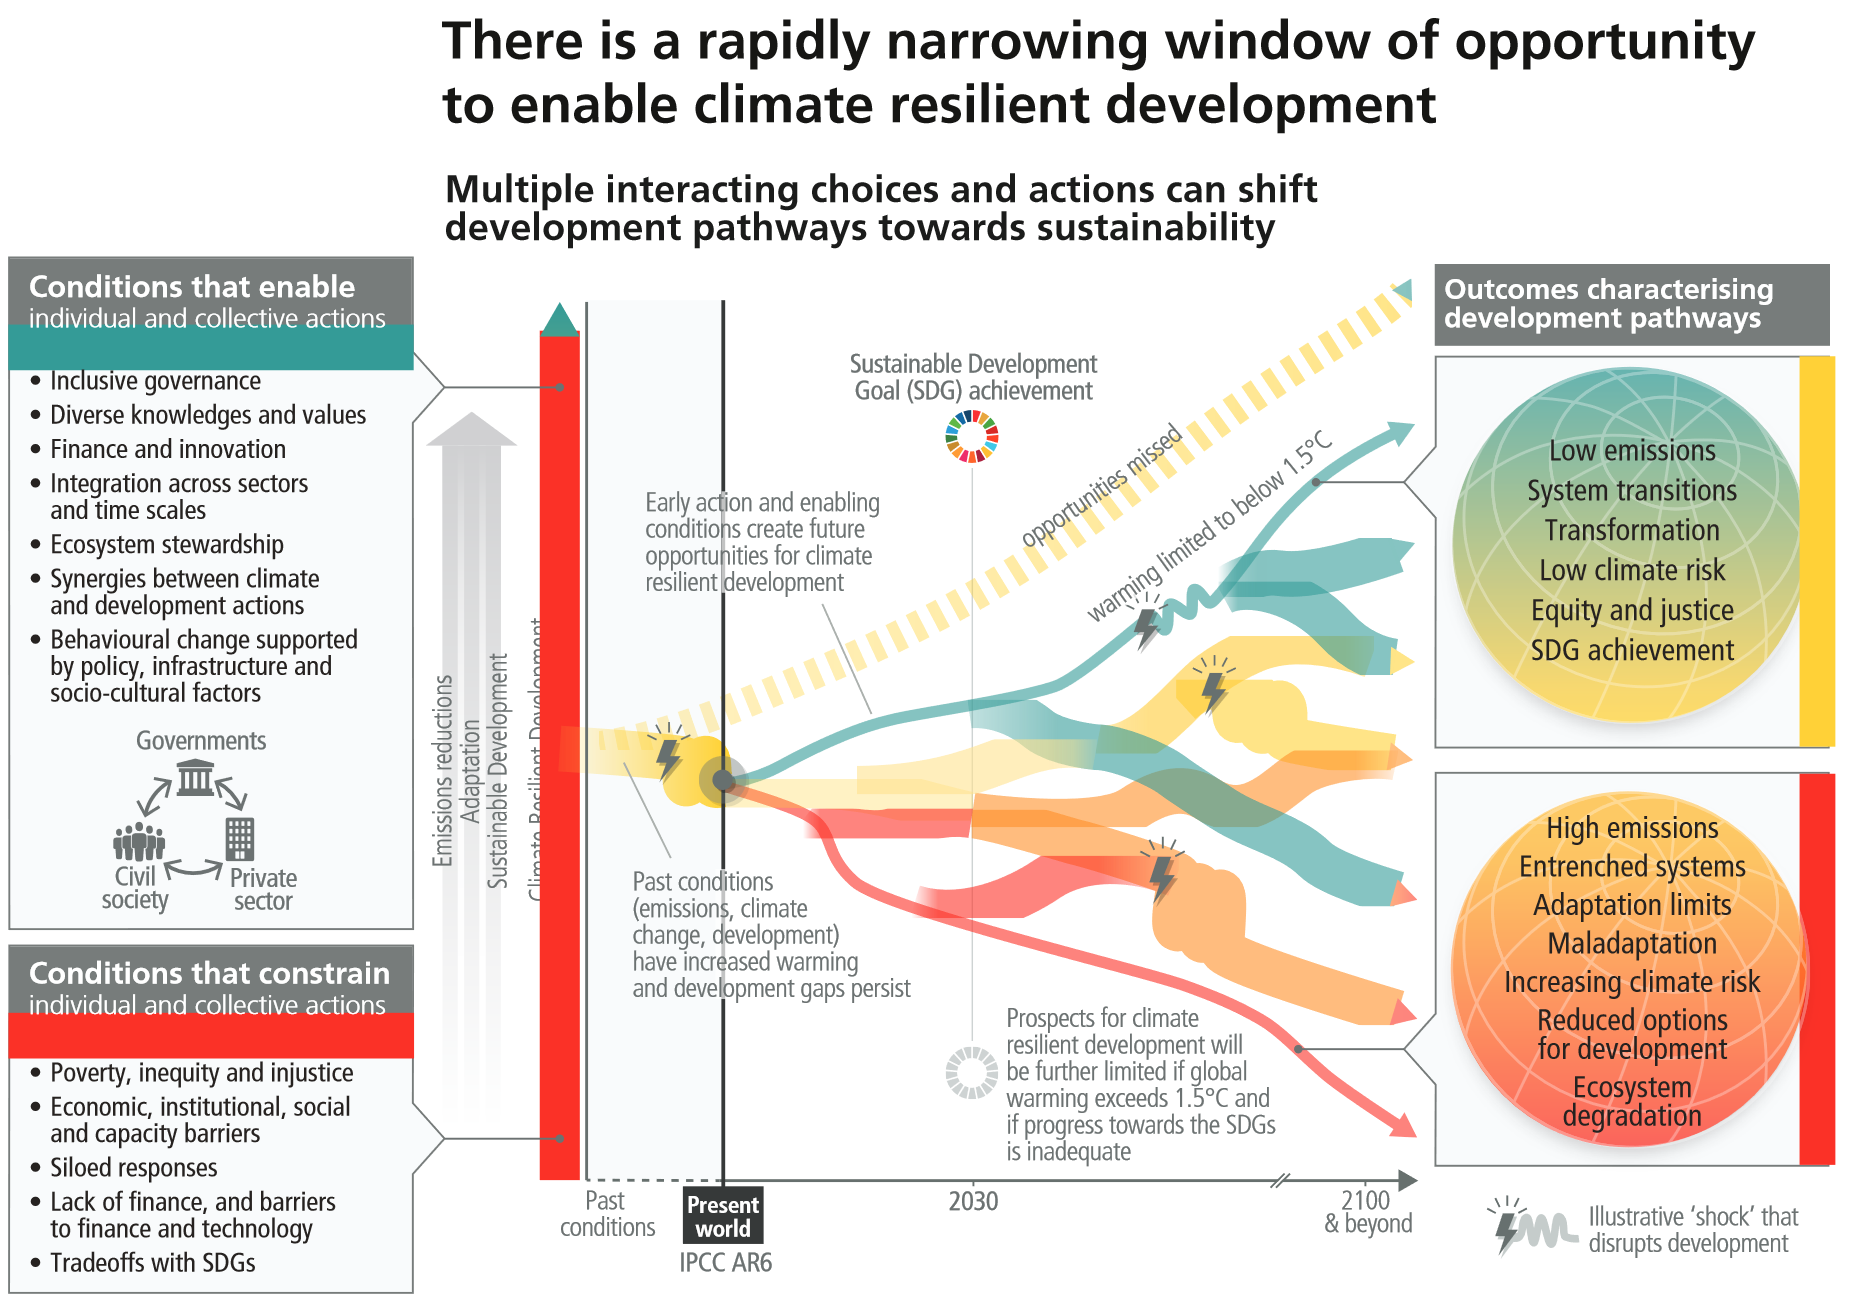
\includegraphics[width=\linewidth]{figures/trajectoire_spm6.png}
    \legende{Les trajectoires possibles pour atteindre les objectifs de développement durable}{Chaque fléche représente symboliquement un chemin de développement possible. Plus les flèches sont rouges, et plus le développement est loin des Objectifs de développement Durable et vulnérable aux aléas climatiques. Cette figure, issue du rapport de synthèse du GIEC (SPM.6) \textcite{lee_ipcc_2023}, montre que les décisions prises aujourd'hui influe les trajectoires possible demain. Elle illustre comment les concepts de trajectoires et de scénarios sont centraux dans le choix du chemin de développement.}
    \label{fig:pathways}
\end{figure}

Si l'existence de celui-ci ainsi que l'ampleur des conséquences qu'il induit ne font plus de doute, les actions à mettre en œuvre et les choix à faire pour le limiter et s'en protéger sont moins consensuelles. Elles font l'objet de nombreux débats, aux niveaux nationaux mais aussi internationaux dans la diplomatie climatique. Un des défis de ces décisions est l'incertitude qui les entoure : on ne connait pas les conséquences de chaque décision, et pourtant, il faut choisir un chemin. Une discipline cherche à éclairer cette route sombre, à la manière des phares d'une voiture : la prospective. Un outil particulièrement utilisé pour réduire cette incertitude est la modélisation, et particulièrement la modélisation intégrée. \\

%% Définition des termes

Pour aborder ce sujet, nous allons mobiliser plusieurs concepts, que nous serons amenés à redéfinir au fil de nos réflexions. 

% Modélisation 

D'abord, celui de \gls{modelisation}. Il s'agit d'une simplification de la réalité, qui permet de mieux la comprendre. Nous nous intéresserons particulièrement aux \gls{iam}, \textit{représentations simplifiées de systèmes sociaux et physiques complexes, qui se concentrent sur les interactions entre l'économie, la société et l'environnement}. Plus simple que les modèles climatiques, ils représentent à la fois des composantes physiques, économiques et énergétiques. Ils permettent ainsi de considérer simultanément ces sous-systèmes et leurs interactions. Les impacts du changement climatique représentent les effets délétères du changement climatique sur les sociétés ou les écosystèmes. 

% Responsabilité / choix / éthique / incertitude



%% Rappel du sujet

Nous nous intéressons donc ici à la modélisation des impacts du changement climatique, c'est-à-dire à la manière dont ils sont représentés dans les modèles intégrés. La question de recherche principale est : faut-il représenter les impacts du changement climatique dans les modèles ? Nous cherchons à y répondre par les sous-questions suivantes : Avec quel niveau de complexité faut-il représenter les interactions entre les sociétés et le climat ? Comment représenter les impacts-non monétaires ? Quelle est la responsabilité des modélisateur.ices sur l'interprétation qui est faite des modèles ?  \\

%% Plan 

\begin{figure}
    \centering
    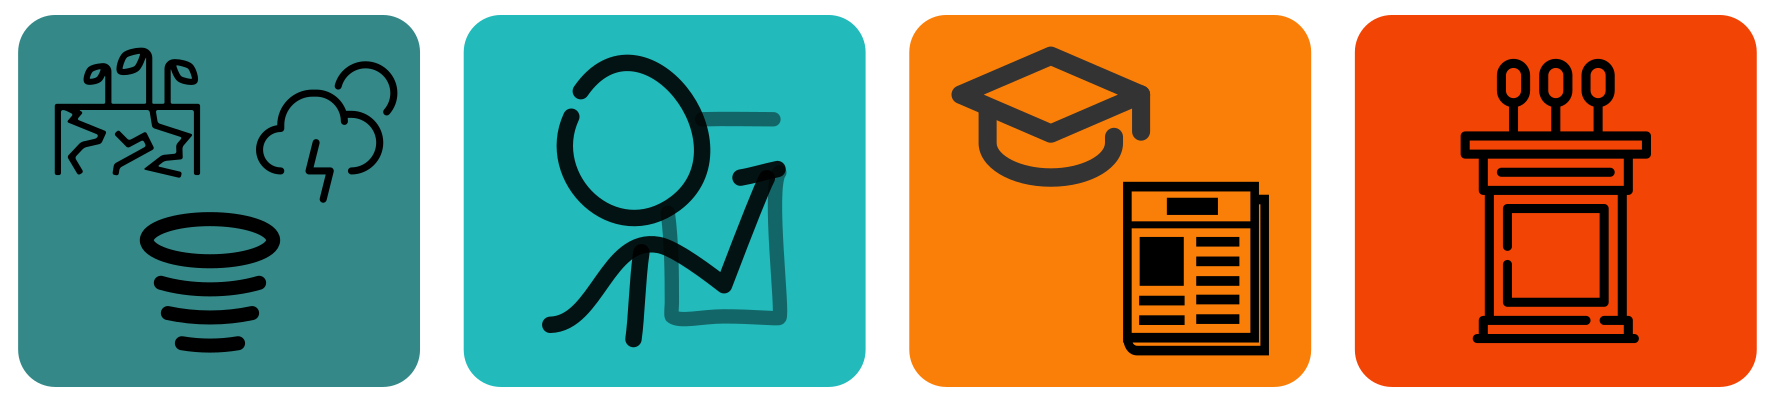
\includegraphics[width=\textwidth]{illustrations/intro.png}
    \legende{Les grandes étapes de la vie d'une modèle}{La modélisation consiste à représenter de manière simplifiée des phénomènes. Dans notre cas, il s'agit de phénomènes liés au changement climatique. Il existent avant toute forme de représentation (A), puis font l'objet d'une simplification (B). Ils sont ensuite interprétés (C), avant de conduire à des actions, telles que des décisions politiques (D). Chacune de ces étapes correspond à un chapitre : d'abord, on commence par évoquer les différents phénomènes qui sont modélisés (\ref{chapter:introduction}), puis on cherche à savoir comment ceux-ci sont représentés (\ref{chapter:litrev}). On analyse ensuite l'importance du choix de représentation sur les interprétations possibles (\ref{chapter:modelisation}), avant de discuter des enjeux éthiques liés à l'interprétation des résultats des modèles (\ref{chapter:ethique}). Enfin, on s'intéresse à la manière dont cette chaîne de production de connaissance alimente le débat public (\ref{chapter:socio}).}
    \label{fig:enter-label}
\end{figure}



Le  chapitre \ref{chapter:introduction} est consacré à une présentation du contexte scientifique et politique dans lequel s'inscrivent les \gls{damage function}. Il présente d'abord les différents risques climatiques, c'est-à-dire les raisons pour lesquelles on s'intéresse au changement climatique. Il poursuit en présentant l'intrication entre les sciences dures et la politique dans les négociations climatiques. Enfin, il présente les outils qui permettent d'éclairer ces décisions, notamment les modèles intégrés et leurs fonctions de dommage. Il sert avant tout à contextualiser l'environnement dans lequel se situe la modélisation intégrée. \\

Le chapitre \ref{chapter:litrev} présente une revue de littérature sur les \gls{damage function}. Il vise à présenter un état des lieux, qui se veut le plus complet mais non exhaustif, des fonctions de dommages qui sont utilisées (ou non) dans les modèles. Il est suivi d'une analyse de cet état des lieux, en classant les fonctions de dommages selon leur utilisation finale, leur forme ou encore les paramètres qui sont pris en compte. \\

Le chapitre \ref{chapter:modelisation} est la partie la plus expérimentale du mémoire. On cherche à quantifier l'effet des choix de modélisation sur le résultat des modèles, c'est-à-dire à quel point ils sont sensibles à leurs hypothèses. Dans un premier temps, on décrit la méthodologie pour pouvoir comparer les différentes fonctions entre elles, puis on réalise de nombreuses simulations avec de légères variations. Ces résultats font ensuite l'objet d'une analyse économétrique, pour quantifier l'effet des variations sur le niveau de dommage final et sa distribution. Cette expérimentation se fait dans le modèle \Gls{WILIAM}, auquel on a ajouté des fonctions reproduisant le comportement des fonctions de dommage d'autres modèles. \\

Dans le chapitre \ref{chapter:ethique}, on identifie des enjeux éthiques liés à la modélisation intégrée, que l'on tente d'éclairer à travers une approche épistémologique. Des exemples, tels que le choix de la forme, de la fonction, des paramètres ou encore des phénomènes représentés, sont analysés grâce à des philosophes des sciences. \\


Le chapitre \ref{chapter:socio} s'interroge sur la perception de ces enjeux éthiques chez les personnes qui participent au débat public sur les questions climatiques. À travers des entretiens semi-directifs chez une dizaine d'acteurs (scientifiques, techniciens, politiques et société civile), on cherche à établir quelle compréhension des enjeux éthiques transparait dans leur transposition au débat public. 

\begin{tcolorbox}[title=Avertissement]
    L'ensemble du code source utilisé dans le cadre de ce mémoire est accessible en libre accès sur \href{https://github.com/ggenelot/damage-functions-modeling}{ce dépôt github}. Par ailleurs, un des fils conducteurs de ce mémoire est de mener une réflexion épistémologique au plus près du modèle, et notamment du code. Cela est notamment rendu possible par \href{https://damage-functions-modeling.readthedocs.io/en/latest/index.html}{ce blog}, qui permet d'intégrer des morceaux de code. Tout au long du mémoire, des passages feront référence à des morceaux de code et/ou à des analyses qui y sont présentées. Il suffit alors de cliquer sur le lien (voir figure \ref{fig:logo}) pour y avoir accès. Il est également possible de se rendre sur le site en scannant le QR code (voir figure \ref{fig:qrcode}). \\

    \begin{center}
        \begin{minipage}{0.3\textwidth} % Ajustez la largeur selon vos besoins
            \centering
            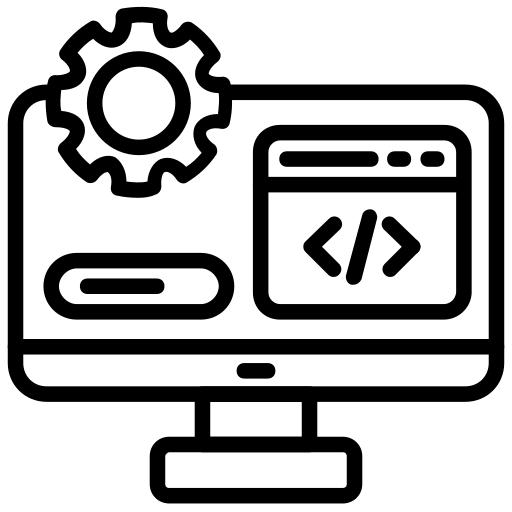
\includegraphics[width=3cm]{figures/logos/development.png}
            \captionof{figure}{Logo cliquable permettant d'accéder au site compagnon}
            \label{fig:logo}
        \end{minipage}%
        \hspace{0.05\textwidth} % Espace entre les deux images
        \begin{minipage}{0.3\textwidth} % Ajustez la largeur du minipage
            \centering
            
\includegraphics[width=3cm]{illustrations/frame.png} % Ajustez la taille du QR code selon vos besoins
            \captionof{figure}{QR code vers le site compagnon}
            \label{fig:qrcode}
        \end{minipage}
    \end{center}



    
\end{tcolorbox}

\begin{tcolorbox}[title=License]
    Toute la production originale est distribué sous la licence CC0. Ceci ne comprend pas les images et figures issues d'autres sources, qui appartiennent à leurs auteurs respectifs. De la même manière, le code source de WILIAM appartient à ses développeurs, et la propriété intellectuelle de chaque fonction de dommage revient à ses créateurs. \\

     \begin{center}
        \begin{minipage}{0.3\textwidth} % Ajustez la largeur selon vos besoins
            \centering
            
\includegraphics[width=6cm]{illustrations/ccby.png}
            \captionof{figure}{Distribué sous licence CC-BY}
            \label{fig:ccby2}
        \end{minipage}%
    \end{center}

\end{tcolorbox}


Les annexes proposent des documents complémentaires, notamment un index / glossaire, qui permet de mieux situés les termes les uns par rapport aux autres. 

